\documentclass[10pt,twocolumn,letterpaper]{article}

\usepackage{cvpr}
\usepackage{times}
\usepackage{epsfig}
\usepackage{graphicx}
\graphicspath{ {images/} }
\usepackage{amsmath}
\usepackage{amssymb}

% Include other packages here, before hyperref.

% If you comment hyperref and then uncomment it, you should delete
% egpaper.aux before re-running latex.  (Or just hit 'q' on the first latex
% run, let it finish, and you should be clear).
\usepackage[breaklinks=true,bookmarks=false]{hyperref}

\cvprfinalcopy % *** Uncomment this line for the final submission

\def\cvprPaperID{****} % *** Enter the CVPR Paper ID here
\def\httilde{\mbox{\tt\raisebox{-.5ex}{\symbol{126}}}}

% Pages are numbered in submission mode, and unnumbered in camera-ready
%\ifcvprfinal\pagestyle{empty}\fi
\setcounter{page}{1}
\begin{document}

%%%%%%%%% TITLE
\title{Automatic Target Scoring}

\author{Ninad Prashant Chaudhari\\
University at Albany\\
{\tt\small nchaudhari@albany.edu}
% For a paper whose authors are all at the same institution,
% omit the following lines up until the closing ``}''.
% Additional authors and addresses can be added with ``\and'',
% just like the second author.
% To save space, use either the email address or home page, not both
\and
Prof. Mei Chen\\
University at Albany\\
{\tt\small meichen@albany.edu}
}

\maketitle
%\thispagestyle{empty}

%%%%%%%%% ABSTRACT
\begin{abstract}
The paper discusses various Computer Vision Techniques that can be used for deducing score from a ISSF 50Meter Rifle Target. The project aims at development of an android application that could use a smartphone's camera to capture video and perform vision on this live video to get the position of a shot and further use the information for scoring. The paper entails various approaches that have been thought of along with details of a few which have been implemented and tested. It was developed as course work for Fall2017 CSI671 under Prof.Mei Chen and Teaching Assistant Lin Zhang. Implementation of ideas as either Matlab code or in the form of an android application has been provided. All source code for the project can be accessed at : \url{https://github.com/ninadpchaudhari/AutomaticTargetScore} 
\end{abstract}

%%%%%%%%% BODY TEXT
\section{Introduction}
\subsection{Mechanics of the Sport}
Rifle shooting is a competitive sport played all over the world and has been played in the Olympic Games since the first modern Olympic Games, Athens, in 1896\cite{ISSFHistory}. The sport is a test of accuracy, precision and speed. One of the recognized sport under shooting domain is 50M Rifle Shooting. 50M Rifle shooting involves a human using a human-portable firearm to aim and then shoot a projectile at a paper target over a distance of 50Meters. The human might be required to shoot in different positions like standing,kneeling or prone depending on the discipline of the competition, but major specifications of rifle, projectile, target remain the same.  The specifications and standards regarding everything in the sport are set forward by the "International Shooting Sport Federation" or ISSF for short. The same association is responsible for management of all shooting related sporting activities on a global level.

Looking at the shooting sport of "ISSF 50M Rifle", ISSF conducts competitions involving 2 major and 2 sub-disciplines, 50M Rifle 3 Position (sub - Men/Women) and 50M Rifle Prone (sub - Men/Women). In all of these events, a human shoots bullet using a rifle. The ammunition that is used for this sport is of ".22LR" specification. This ammunition consists of a solid projectile, primarly made of lead with outer diameter of .22Inches (or 5.588mm) and a case (or shell), primary made of copper which hosts the gun-powder and other necessary projectile required to expel the bullet. This bullet travels a distance little less than 50Meters with sub-sonic speed and finally hits the stationary paper target which consists of concentric rings of increasing radii; the one with least radius scoring the most. Detailed specifications of the target are explained later in this paper. After the paper is hit, it naturally forms a circular punch in the paper.

\subsection{Target and Scoring Technique}
\begin{figure}[h]
	\centering
	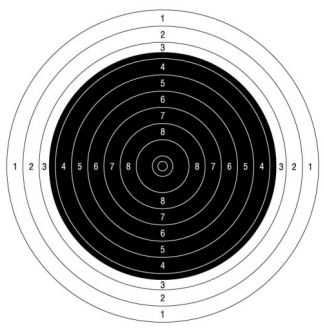
\includegraphics{50mRifleShootingTarget}
	\caption{ISSF 50M Rifle Shooting Target}
\end{figure}

The ISSF target for 50M Rifle shooting target consists of 11 concentric circles each but the last one representing 1 point. Usually all international competitions have electronic scoring systems which have rubber targets and use sound or (more recently) light triangulation for shot placement and hence scoring. Though the use of electronic targets is suitable for National and International competitions, the same cannot be used at other smaller competitions due to the direct installation and further indirect licensing costs. Moreover electronic targets can be damaged by new athletes who might shoot the electronic components in the target during a match. Hence many organizations still rely on humans to do shot placement and scoring of their competitions. Additionally, paper targets see widespread use by athletes during training thanks to the cost. Specifications of the target are as follows\cite{ISSFRuleBook-50MTargetSpecification}
\begin{center}
	\begin{tabular}{ c c }
		\textbf{Ring no.}  & \textbf{Diameter (Tolerance) }\\
		10 Ring & 10.4 mm (±0.1 mm)\\ 5 Ring &  90.4 mm (±0.5 mm)\\ 
		 9 Ring & 26.4 mm (±0.1 mm)\\ 4 Ring & 106.4 mm (±0.5 mm)\\ 
		 8 Ring & 42.4 mm (±0.2 mm)\\ 3 Ring & 122.4 mm (±0.5 mm)\\
		 7 Ring & 58.4 mm (±0.5 mm)\\ 2 Ring & 138.4 mm (±0.5 mm)\\
		 6 Ring & 74.4 mm (±0.5 mm)\\ 1 Ring & 154.4 mm (±0.5 mm)\\	
	\end{tabular}

Inner Ten = 5 mm (±0.1 mm).
Black from part of 3 to 10 rings = 112.4 mm (±0.5 mm).
Ring Thickness: 0.2 mm to 0.3 mm.
\end{center}

In a competition which involves manual scoring, after the athletes complete shooting, the targets are sent to the officials for scoring. Here, each target is scored separately and then the scores of all targets is added up to give a final score. The scoring is done based on the shot placement on target. Score is given based on the innermost area the bullet has hit \eg if the hole's boundary touches the 3rd ring from outside, the score is declared as "3". The region between the rings correspond to the score of the inner ring. Officials may use special inserts which mimic the bullet's diameter in case the bullet did not leave a clean hole and there might be some obstruction due to residual paper.

\subsection{Motivation}
As described earlier, this process of shot placement is done by humans. Not only is the task repetitive, prone to human errors, but it also might be subject to bias. The paper discusses how this process of shot placement can be done by using a smartphone camera which would reduce the cost and make the process much faster. Additionally, Rifle shooting sport is a blooming business and thanks to investments by governments all around the world, the sport is being accessible by more and more individuals everyday.

%------------------------------------------------------------------------
\section{Related Work}

An App called "Target Scan" \cite{TargetScanApp} Exits in the app store which achieves similar results. The application allows the user to click a photo of the target and it tries to get the score of the same. It does support the ISSF 50M target but has closed source code. Moreover, it does not work with video and live shot detection. Apart from that it is an excellent application which seems to work well.
%-------------------------------------------------------------------------
\section{Approach to solve the problem}

The challenges for this problem have been identified as follows and each of these challenges are discussed in every proposed solution.
\begin{itemize}
\item Identify the Target.​

\item Identify the shot placement.

\item Identify the position of shot with respect to some stationary point

\item Tackle Projective and Scaling transformations.​

\item Triangulate position of shot.​

\item Deduce score.
\end{itemize}	

The following list contains the hypothetical solution to the problem:
\begin{enumerate}
\item Detect the small circle ( corresponding to bullet).​

\item Refine the Circle as much as possible.

\item Detect a feature, dimensions of which in physical world are known.
\item Find the amount of pixels that correspond to 1mm

\item Find Distance between the shot center and another feature.

\item Study the standards for the target and formulate an equation for calculating a robust distance measure between the circle and the other larger feature.

\item Make it independent of scale.​

\item Transfer the logic to Mobile device.
\end{enumerate}
\section{Process the Target}
In section we try to separate all the noise and try to find interesting information from the target which is in the background. I am refining the target by using the following steps:
\begin{enumerate}
	\item Gray scale conversion -> Reduce the amount of information to work with and deal with single dimension matrix.
	\item Thresholding -> primitive differentiation between various components and this further allows me to carryout component differentiation.
	\item Determine connected components
	\item Remove the components which have areas less than 140px. (empirical constant obtained by experimentation)
\end{enumerate}
Results are displayed in \ref{TargetPreProcessing}
\begin{figure}[h]
	\centering
	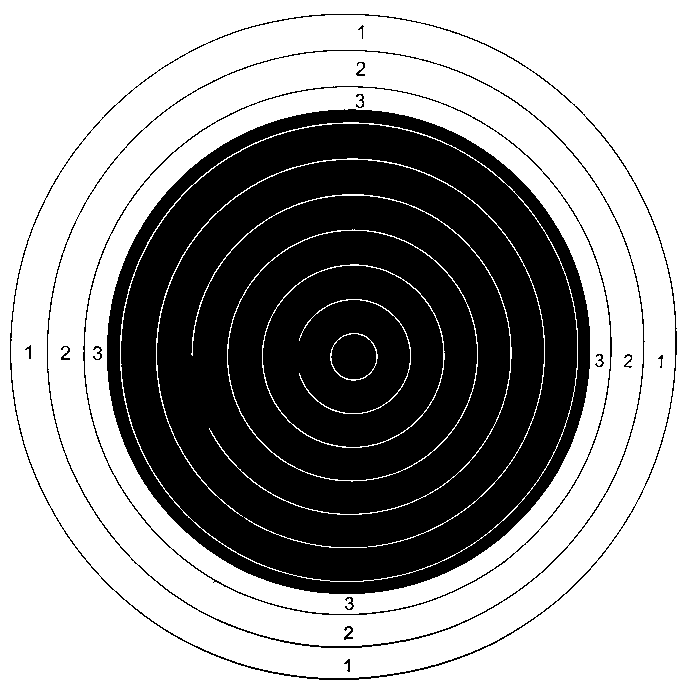
\includegraphics[width=\linewidth]{PreProcessedImage}
	\label{TargetPreProcessing}
	\caption{Target after the processing applied}
\end{figure}

%-------------------------------------------------------------------------
\section{Proposed Solutions for Shot Placement}

One of the major tasks in the project has been to find the position of the hole made by the bullet for an accurate shot placement. Proposed solutions are 
\begin{itemize}
	\item Case Insert Method.
	\item Contrasting background behind the hole.
	\item Finding Contours.
	\item Find all circles using Hough Circles, Then find closest proximity.
	\item Find 1 circle then use it to compute other metrics.
\end{itemize}
\subsection{Find All Hough Circles}
This approach involves trying to find all the circles on the target, then we can calculate the multiplication Factor which we discuss later after target processing and since now we have all the radii of the captured circles, we can compare to the ring sizes and get a measure of the value of the ring. Later use this information to get which ring the shot is close to.

Implementation of this method can be found in the android app 1, but I was not able to optimize it enough to run on a mobile. Even matlab needs significant amount of time to calculate all circles. I later wrote another app (Android app 2) where I try to capture a single photo and then try to perform this operation. But since the other methods work better and since the whole point of this project was to find scores in live video, the same was rejected.
\subsection{Find 1 circle method}
Similar to the earlier approach, just find only 1 circle by giving appropriate radius range to the hough circle function.
\begin{figure}[h]
	\centering
	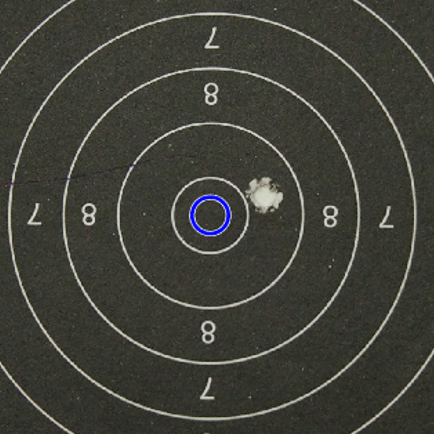
\includegraphics[width=\linewidth]{oneRing}
	\caption{1 ring found by hough}
\end{figure}

\begin{figure*}[!h]
	\centering
	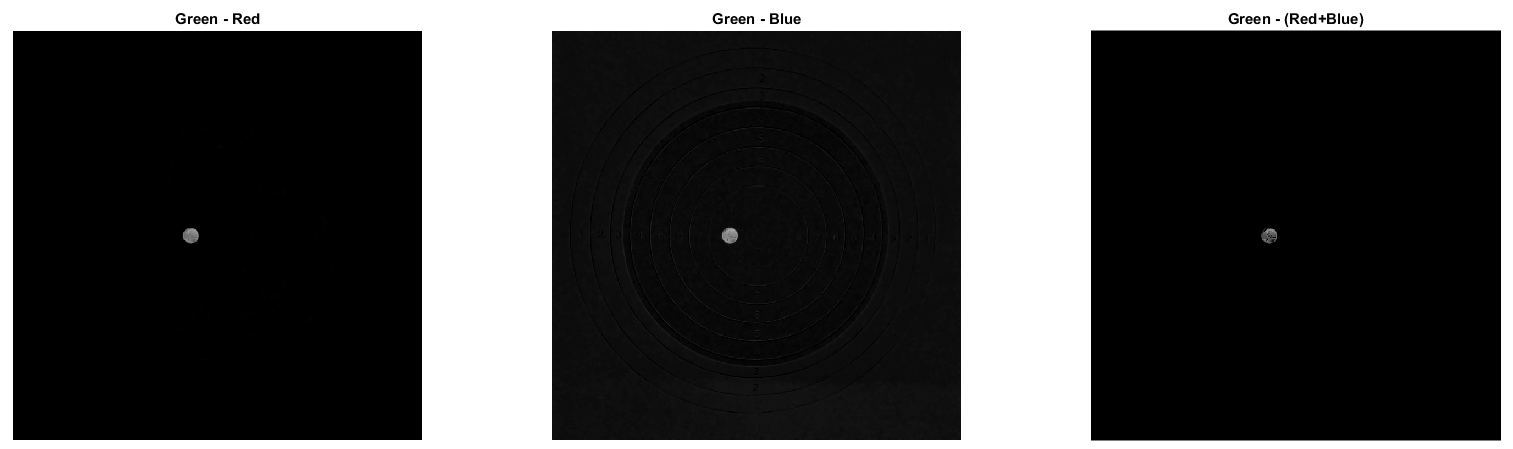
\includegraphics[width=\textwidth]{BulletPositionExtraction}
	\caption{From the Right to Left, green-red , green-blue, green-(Red+blue) channels of the case insert image}
	\label{BulletPositionExtractionImage}
\end{figure*}
\subsection{Case Insert Method}
This method involves inserting a empty case obtained from the bullet in the hole.
This results in the hole stretching out and hence it solves the problem of improper hole formation and removes obstruction caused by paper. The case so inserted can also have a distinctive color like Green so that we can easily do background subtraction to obtain the precise location of the bullet on the frame.
\begin{figure}[h]
	\centering
	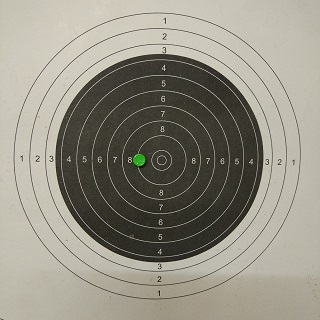
\includegraphics[width=0.5\textwidth]{CaseInsertImage}
	\caption{Image of a Target with Case Insert. The case is green in color.}
	\label{CaseInsertImage}
\end{figure}
I tried with other color inserts like White, but green was chosen since it is one of the fundamental colors and it would be easier to distinguish it from the image background. Additionally, I found green channel had the lowest noisy information. i.e. after a red insert, the result does look fine in red channel, but there are traces of a lot of image parts in the channel along with the bullet location pixels.

As seen in the image-\ref{BulletPositionExtractionImage}, I checked out various combinations instead of just green channel - red+blue channels. Though Green-blue seem to give pretty good circle of the green case, we can see a lot of other information as well. Instead, completely removing other channels from green gives us an image that we can use connected components and further morphological operations to further enhance the image.
\begin{figure}[h]
	\centering
	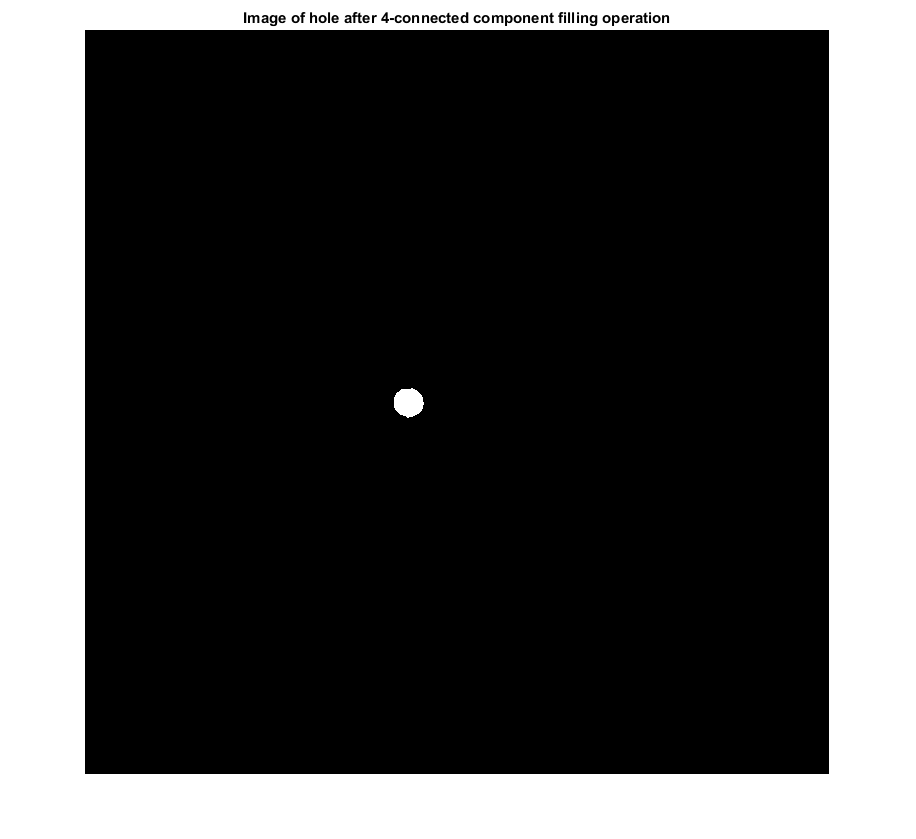
\includegraphics[width=0.5\textwidth]{OnlyGreenAfterRefine}
	\caption{We get awesome result of just green pixels after we do 4-pixel connected components filling and then closing operation}
	\label{OnlyGreenAfterRefine}
\end{figure}
As seen in \ref{ShotCentroid}; We Further locate the centroids of this component and plot it beside the centroid of the black circle component which we obtain from the method mentioned in the section of target processing.
\begin{figure} 
	\centering
	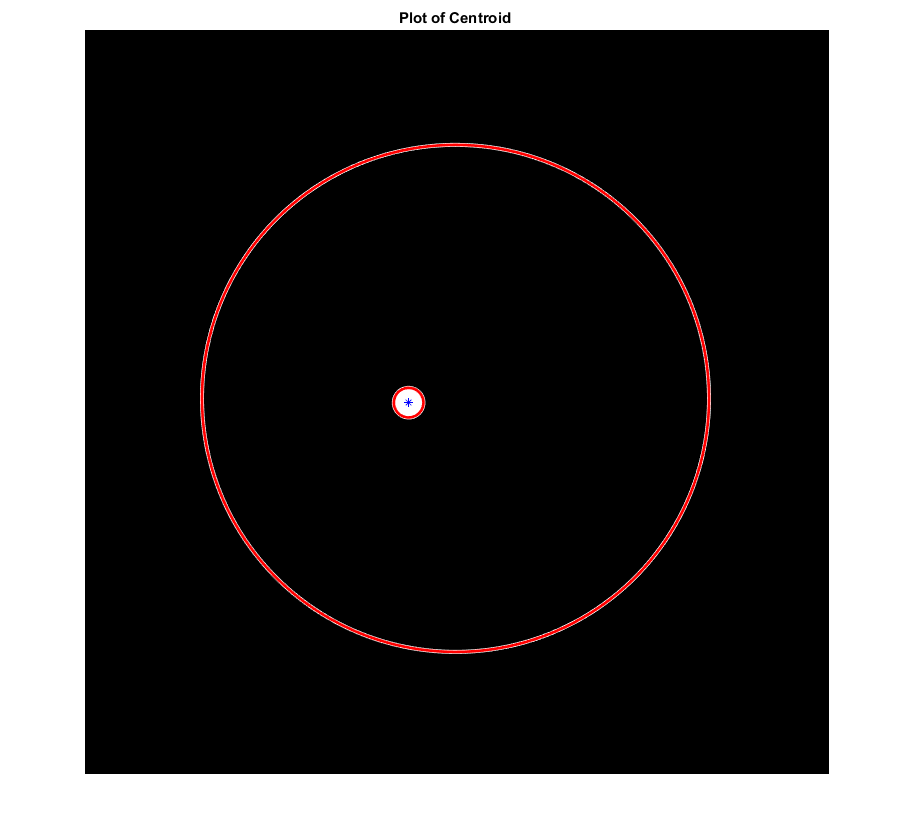
\includegraphics[width=\linewidth]{ShotCentroid}
	\caption{Plotting centroid of the shot over outline of black region of target}
	\label{ShotCentroid}
\end{figure}
Now that we have the centers of these 2 circles, we find the distance between the centers using distance formula.
This distance can be multiplied by the multiplication factor which is obtained by
\[\ 1px = 112.4(mm)/DiameterOfBlackCircle(px) \] Since 112.4mm is the physical diameter of the black circle. We then convert the distance in pixel to distance in mm by multiplying the distance to the multiplication factor.
\subsection{Correctness Measure}
After we get the centers and radii of these circles, we obtain the correction ratio (correctnessFactor)
\[
correctnessFactor = \frac{Diameter Of Black Circle (px)}{Diameter Of Case Brim (px)}
\]
Since the ratio removes the factor of Pixels, it must match the actual ratio of Diameter Of Black circle / Diameter of Case Brim in mm.
"real diameter of black circle" and "real diameter of the case's edge". This number will assure us that the kernels we chose for operations did not over eat the image and make it inaccurate. It is a important metric which can be used to compare implementation performances in terms of accuracy 
\subsection{Contrasting Background behind Hole}

We can place the target to be scored on a green background and hence use the same techniques mentioned earlier to get the approximate location of the hole and further refine the shot hole by using the morphological operations as mentioned earlier.
If this method is used, we risk in loosing too much accuracy and hence the corretnessFactor as mentioned earlier would deviate too much from the actual.

We can use the target processing as mentioned later and then estimate the radius of the corresponding hole since the diameter of the bullet is .22Inches. This way we have a known circle which can try and fit in the obtained hole boundary points and further increase accuracy of shot placement.
\subsection{Using Contours}
We can use the built-in function to find contours and hence use the above mentioned techniques. This function use the paper : S. Suzuki and K. Abe. Topological structural analysis of digitized binary images by border following. CVGIP, 30(1):32–46, April 1985.
To find connected edges.
\begin{figure}[h]
	\centering
	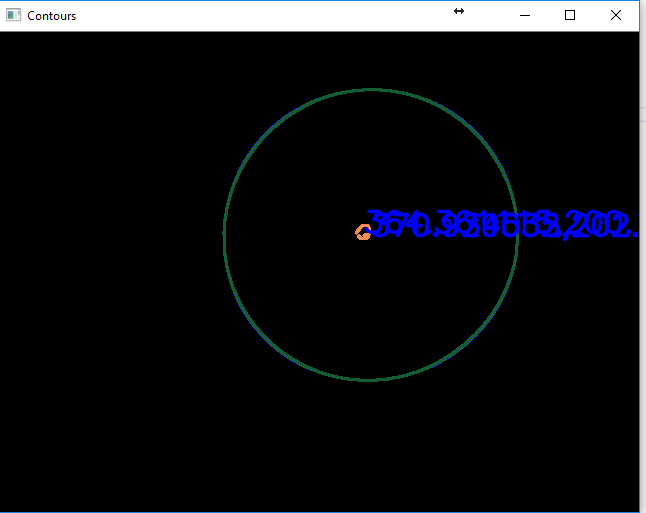
\includegraphics[width=0.5\textwidth]{contour}
	\caption{Image with centers of the outer ring and the inner shot}
	\label{contourImage}
\end{figure}
\section{Conclusion}

Various techniques have been discussed for shot placement and score deduction. Further work can be done to develop an android app with good UI based on the concepts.
The Shot Insert method is the one I spent most time on and it followed by the findContour method seem to have best results.

{\small
\bibliographystyle{ieee}
\bibliography{egbib}
}

\end{document}
